% \begin{figure*}[t]
%     \centering
%     \captionsetup{font={small}}
%     \includegraphics[width=\linewidth]{asset/sim2sim_eval_all.pdf}
%     % \vspace{-10pt}
%     \caption{\textbf{Average performance on sim-and-sim experiments.} We can find that alignment-based methods (+OT/+ADDA) get improvement in the balanced mixing ratio group, while discernibility-based methods (+CFG) get improvement mainly in the unbalanced mixing ratio group. More detailed results are available in the Appendix.~\ref{appdx: sim2sim detailed results}}
%     \label{fig: sim2sim eval}
%     % \vspace{-20pt}
% \end{figure*}

\begin{figure*}[t]
    \centering
    \captionsetup{font={small}}
    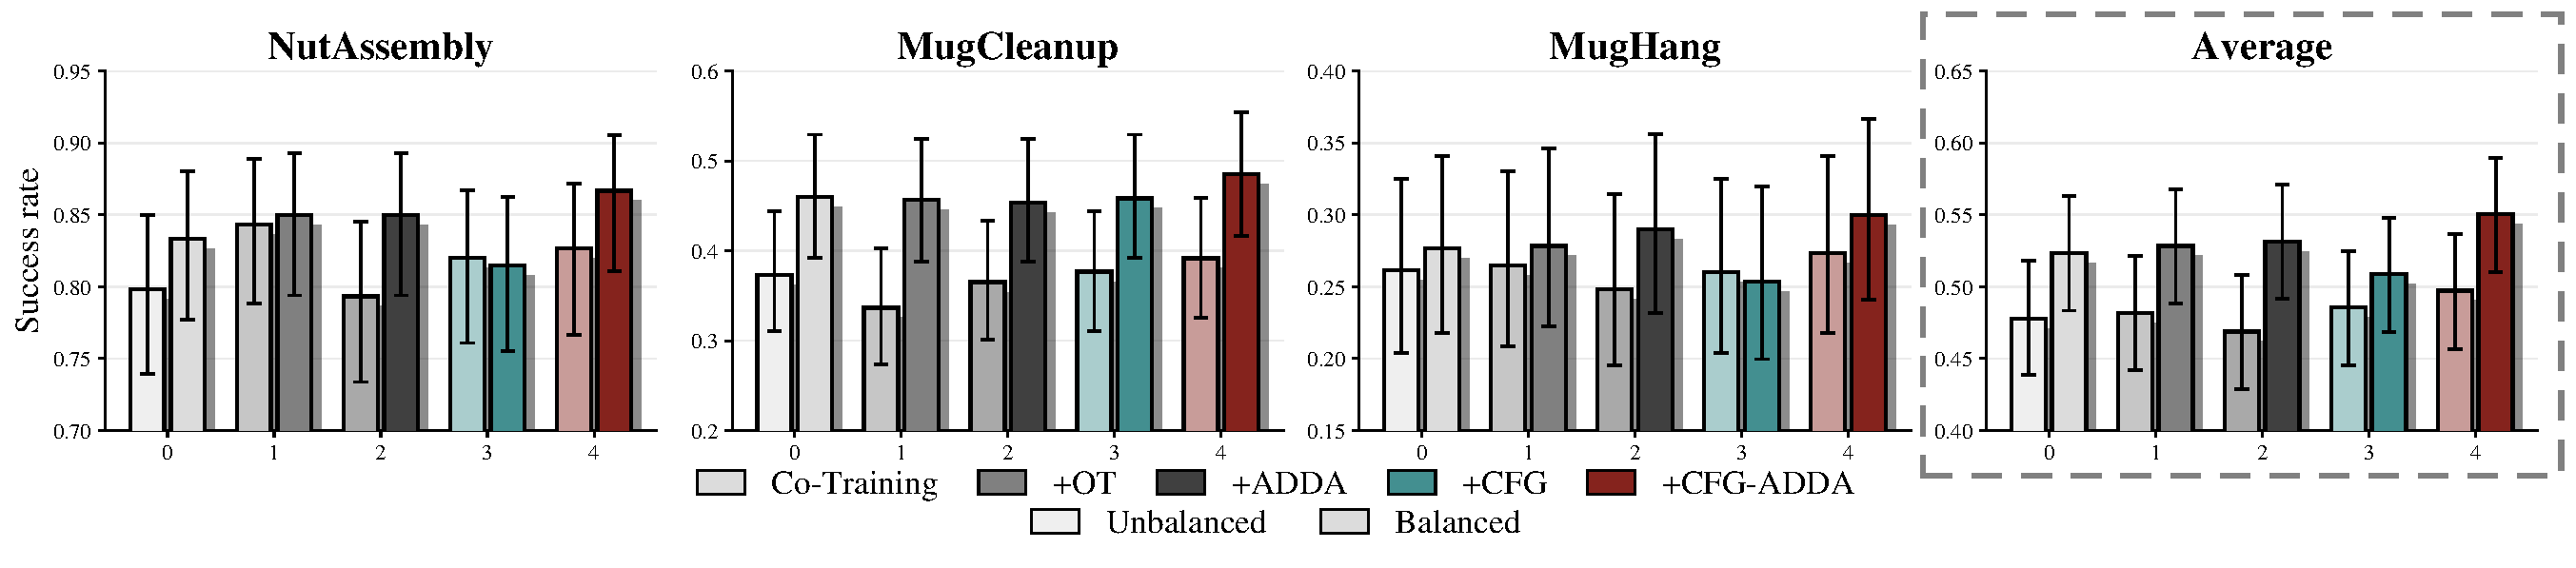
\includegraphics[width=\linewidth]{asset/sim2sim_eval_all2.pdf}
    % \vspace{-10pt}
    \caption{\textbf{Average performance on sim-and-sim experiments.} We can find that alignment-based methods (+OT/+ADDA) get improvement in the balanced mixing ratio group, while discernibility-based methods (+CFG) get improvement mainly in the unbalanced mixing ratio group. More detailed results are available in the Appendix.~\ref{appdx: sim2sim detailed results}}
    \label{fig: sim2sim eval}
    % \vspace{-20pt}
\end{figure*}

\begin{table*}[t]
\centering
\small
\setlength{\tabcolsep}{6pt}
\begin{tabular}{l ccc ccc ccc c}
\toprule
\multirow{2}{*}{\textbf{Method}} 
& \multicolumn{9}{c}{\textbf{Success Rate}} 
& \multirow{2}{*}{\textbf{Avg}} \\
\cmidrule(lr){2-10}
& \multicolumn{3}{c}{\textbf{NutAssembly}} 
& \multicolumn{3}{c}{\textbf{MugCleanup}} 
& \multicolumn{3}{c}{\textbf{MugHang}} 
&  \\
\cmidrule(lr){2-4} \cmidrule(lr){5-7} \cmidrule(lr){8-10}

% ---------------- Real-only ----------------
Real-only
& \multicolumn{3}{c}{11/30}
& \multicolumn{3}{c}{8/30}
& \multicolumn{3}{c}{6/30}
& 8.6/30 \\

% ---------------- Mixing ratio ----------------
\midrule
Mixing Ratio $w$
& 0.016 & 0.1 & 0.3
& 0.016 & 0.1 & 0.3
& 0.016 & 0.1 & 0.3
& - \\

% ---------------- Co-training ----------------
\midrule
Co-Training
& \cellcolor{ylog}\textbf{17/30} & 11/30 & 16/30
& \cellcolor{ylog}\textbf{16/30} & 9/30 & 7/30
& 8/30 & \cellcolor{ylog}\textbf{13/30} & 7/30
& 15.3/30 \\

\midrule
\quad + OT
& 15/30 & \cellcolor{ylog}\textbf{17/30} & 11/30
& 8/30 & 15/30 & \cellcolor{ylog}\textbf{15/30}
& \cellcolor{ylog}\textbf{11/30} & 9/30 & 4/30
& 14.3/30 \\

\quad + ADDA
& \cellcolor{ylog}\textbf{13/30} & 13/30 & 15/30
& 6/30 & \cellcolor{ylog}\textbf{14/30} & 11/30
& 10/30 & \cellcolor{ylog}\textbf{14/30} & 7/30
& 14.3/30 \\

\quad + CFG
& \cellcolor{ylog}\textbf{15/30} & 14/30 & 11/30
& 6/30 & \cellcolor{ylog}\textbf{17/30} & 14/30
& 8/30 & \cellcolor{ylog}\textbf{14/30} & 10/30
& 15.3/30 \\

\midrule
\textbf{+ CFG-ADDA($\lambda=0$)}
& \cellcolor{ylog}\textbf{20/30} & 17/30 & 11/30
& 15/30 & \cellcolor{ylog}\textbf{19/30} & 14/30
& 15/30 & \cellcolor{ylog}\textbf{17/30} & 13/30
& \cellcolor{ylog}\textbf{18.6/30} \\

\textbf{+ CFG-ADDA($\lambda=-0.5$)}
& \cellcolor{ylog}\textbf{23/30} & 15/30 & 18/30
& 11/30 & \cellcolor{ylog}\textbf{22/30} & 17/30
& \cellcolor{ylog}\textbf{18/30} & 15/30 & 8/30
& \cellcolor{ylog}\textbf{21/30} \\

\bottomrule
\end{tabular}
\caption{
\textbf{Real-world policy performance under different co-training strategies.}
}
\label{tab: real_world_eval}
\vspace{-10pt}
\end{table*}

% \begin{table*}[ht]
% \centering
% % \vspace{-0.5em}
% % \vspace{-1em}
% \resizebox{\linewidth}{!}{
% \begin{tabular}{l|c|c|c|c|c|c|c|c|c|c}
%     \toprule
%                             &Nut Assembly1    &Nut Assembly2    &Nut Assembly3   &Mug Cleanup1    &Mug Cleanup2    &Mug Cleanup3  &Mughang1    &Mughang2     &Mughang3  &Avg   \\
%     \midrule
%      Real-Only &  372.35     &  372.35     & 372.35  &  372.35     &  372.35     & 372.35 &  372.35     &  372.35     & 372.35    &  0.337    \\
%      \midrule
%      Vanilla Co-Training &  0.305     &  0.316     & 0.324 &  0.305     &  0.316     & 0.324  &  0.305     &  0.316     & 0.324     &  0.337    \\
%     \midrule
%     + Adversarial    & 372.35      &  315.15    & 301.54 & 372.35      &  315.15    & 301.54  & 372.35      &  315.15    & 301.54   &  496    \\
%     \midrule
%     + OT    & 372.35      &  315.15    & 301.54 & 372.35      &  315.15    & 301.54 & 372.35      &  315.15    & 301.54    &  496    \\
%     \midrule
%     + One-hot Condition    & 372.35      &  315.15    & 301.54 & 372.35      &  315.15    & 301.54 & 372.35      &  315.15    & 301.54   &  496    \\
%     \bottomrule
% \end{tabular}
% }
% \caption{Real-world Evaluations (Place Holder now, needs reformatting). 3 different mixing ratios for each task.}
% % \vspace{+.5em}
% % \captionsetup{font={tiny}}
% \label{tab:real-world evaluations}
% % \vspace{-0.3em}
% \end{table*}



\section{A Unified View of Co-Training Methods}
Although a wide range of co-training techniques has been proposed, it often remains unclear why these methods yield performance gains in some settings while failing in others.
In this section, we revisit three representative co-training approaches through the lens of our findings and show that their empirical behavior can largely be explained by how they balance representation alignment and domain discernibility.
Specifically, we categorize existing methods based on whether they primarily promote cross-domain alignment or preserve domain-specific information.

\subsection{Prior Co-Training Methods}

\textbf{Optimal transport (OT)}~\cite{courty2016optimal}-based methods aim to align simulation and real-world data by explicitly matching their representation distributions, either in latent or trajectory space.
Recent work~\cite{punamiya2025egobridge, cheng2025generalizable} formulated co-training as a joint optimal transport problem, in which samples from simulation and real domains are softly coupled to minimize a global discrepancy:
\begin{equation}
    \min_{\phi,\theta} L_w(\phi, \theta) + \lambda\cdot L_{OT}(D_r, D_s).
\end{equation}
% \textcolor{red}{If you are going to show equations, which is not completely necessary here, make sure all symbols are defined!}
$L_{OT}$ is usually computed using the Wasserstein distance between two domains. Under our hypothesis, such methods strongly encourage representation overlap across domains, effectively pushing simulation and real observations into a shared latent space.
We implement OT-regularized co-training as in \citet{cheng2025generalizable}, and the only difference is that we drop the offline data pairing sampler.

\textbf{Adversarial domain adaptation (ADDA)} methods~\cite{tzeng2017adversarial, cai2025n} similarly seek domain-invariant representations by training a discriminator to distinguish between simulation and real data, while simultaneously learning an encoder that attempts to fool the discriminator:
\begin{equation}
    \min_{\phi,\theta} L_w(\phi, \theta) + \lambda\cdot L_{disc}(D_r, D_s).
\end{equation}
% \textcolor{red}{Same comment as above}
$L_{disc}$ can be implemented simply using binary cross-entropy loss.
% Classic domain adaptation approaches follow the same principle, implicitly assuming that domain-invariant features are sufficient for downstream control.
From the perspective of our hypothesis, adversarial alignment also prioritizes cross-domain overlap, but does so implicitly through representation indistinguishability rather than explicit distribution matching.
We implement it in the same way as \citet{tzeng2017adversarial}.


\textbf{Classifier-free guidance (CFG)}~\cite{ho2022classifier} introduces a distinct mechanism for co-training by interpolating between conditioned and unconditioned policies at inference time.
Rather than enforcing representation alignment during training, CFG modulates the influence of real-derived signals via a guidance scale.
Under our hypothesis, CFG preserves domain discernibility by maintaining separate conditional pathways, while still enabling controlled knowledge transfer from simulation:
\begin{equation}
    \tilde{s}_\theta (a,o,c,t) = (1+\lambda)\cdot s_\theta(a,o,c,t) - \lambda \cdot s_\theta(a,o,\varnothing,t).
\end{equation}
We implement it by concatenating a one-hot embedding $c$ as environment labels to the observation features after the vision encoder, setting $\lambda$ to $0$ as recommended in \citet{wei2025empirical}.

\textbf{CFG-ADDA: a simple combination.}
Viewed through our explanation framework, existing co-training methods primarily differ in how they trade off representation alignment and domain discernibility.
OT and ADDA-based methods emphasize alignment, which can be beneficial when domain discrepancies are small but may lead to negative transfer when discrepancies are large.
In contrast, classifier-free guidance preserves domain awareness while allowing flexible information sharing.
This unified perspective clarifies the strengths and limitations of prior approaches and motivates our proposed combination strategy, which explicitly balances these two competing objectives.
We simply combine the techniques of \textit{CFG} and \textit{ADDA}, named as \textit{CFG-ADDA}. Specifically, we attach one-hot embeddings as environment labels to enable domain guidance, while encouraging the remaining representation dimensions to align through an adversarial discriminator. 
Training details are provided in Appendix~\ref{appdx: training details}.

With this explicit disentanglement of domain-invariant and domain-specific features, we want to point out a new perspective towards the score interpolation coefficient $\lambda$ --- as only the environment labels are dropped in $s_\theta(a,o,\varnothing,t)$, it actually represents the average log-probability gradient direction in all domains.
So $\lambda$ can be viewed as a more flexible control variable to transfer the ``averaged knowledge" during inference as opposed to transferring during training by importance reweighting effect.
We set $\lambda=-0.5$ for \textit{CFG-ADDA} as default.

\begin{figure}[htbp]
    \centering
    \captionsetup{font={small}}
    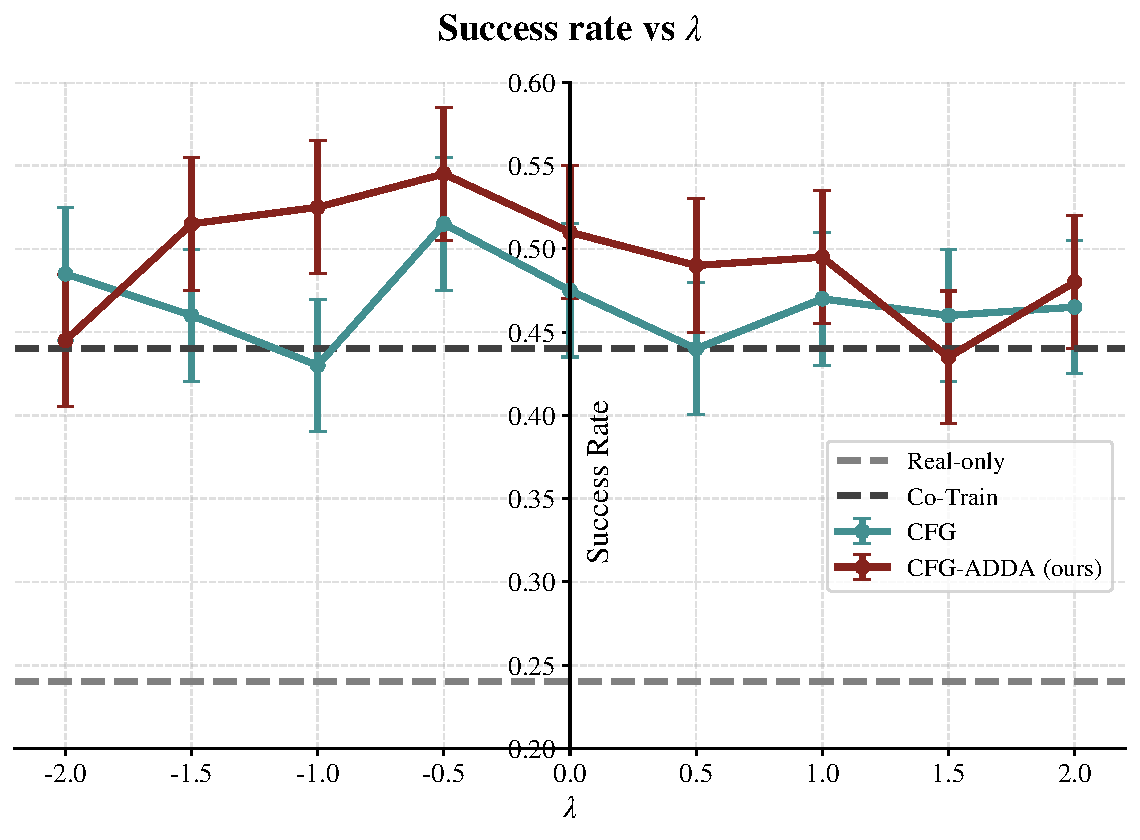
\includegraphics[width=0.98\linewidth]{asset/guidance_scale_ablation.pdf}
    % \vspace{-10pt}
    \caption{\textbf{Performance of different co-training methods on \textit{MugCleanup} with $w=0.1$ in sim-and-sim settings.} The plots are similar for all tasks and balanced mixing ratios.}
    \label{fig: ablations}
    \vspace{-10pt}
\end{figure}


\subsection{Experiments and Analysis}

\textbf{Sim-and-Sim Experiments.}
We implement the above techniques on top of our co-training model and conduct visual-physics sim-and-sim co-training experiments.
The results are shown in Fig.~\ref{fig: sim2sim eval}.
We group the data mixing ratios into two regimes: balanced and unbalanced mixing.
Performances with balanced mixing ratios are consistently better than with unbalanced mixing ratios.
Under balanced mixing, where simulation and real data are present in comparable proportions, alignment-oriented methods (OT and ADDA) consistently improve performance across tasks.
This indicates that representation alignment effectively facilitates cross-domain knowledge transfer when both domains are sufficiently observed during training.
In contrast, under unbalanced mixing, alignment-only methods exhibit pronounced performance degradation, particularly on \texttt{MugCleanup} and \texttt{MugHang}.
This behavior suggests that when one domain dominates the training data, enforcing strong alignment biases the learned representation toward suboptimal invariances, thereby hindering real-world adaptation.
CFG, which explicitly preserves domain information, demonstrates greater robustness in this regime, but its peak performance remains limited.
Notably, CFG-ADDA achieves strong performance across both regimes.
By combining adversarial alignment with explicit domain conditioning, it leverages transferable structure from simulation under balanced mixing while maintaining domain discernibility under unbalanced mixing.

\textbf{Sim-and-Real Experiments.}
Since balanced mixing ratios are the main choice for effective co-training, we conduct real-world evaluations only in this regime.
The observations in the Table~\ref{tab: real_world_eval} are similar to sim-and-sim settings.
We even find more stable and substantial improvement with our proposed method in the real world, achieving $\sim74\%$ success rate on these challenging tasks.

\textbf{Ablations on Guidance Scale.}
In contrast to using only the positive values, we sweep $\lambda$ in the interval of $(-2,2)$ with both \textit{CFG} and \textit{CFG-ADDA}. 
As shown in Fig.~\ref{fig: ablations}, our proposed method consistently outperforms \textit{CFG} with different guidance scales.
Besides, both methods exhibit improvement with $\lambda=-0.5$.
So instead of setting $\lambda>0$ to amplify the action gaps in a traditional way, we advocate setting $\lambda<0$ to actively transfer knowledge from the surrogate domains during inference.




These results support our findings that effective sim-and-real co-training requires both representation alignment for transfer and domain discernibility for adaptive behavior.







